\documentclass[sigchi]{acmart}

\def\tightlist{}
\settopmatter{printacmref=false}
\renewcommand\footnotetextcopyrightpermission[1]{}
\settopmatter{printfolios=true}

$if(highlighting-macros)$
$highlighting-macros$
$endif$

\usepackage{booktabs} % For formal tables

% Copyright
\setcopyright{none}
%\setcopyright{acmcopyright}
%\setcopyright{acmlicensed}
%\setcopyright{rightsretained}
%\setcopyright{usgov}
%\setcopyright{usgovmixed}
%\setcopyright{cagov}
%\setcopyright{licensedcagov}
%\setcopyright{cagovmixed}
%\setcopyright{licensedothergov}

% DOI
\acmDOI{10.475/123_4}

% ISBN
\acmISBN{123-4567-24-567/08/06}

%Conference
\acmConference[Business Intelligence]{Assignment 3}{January 2021}{Linz/Vienna, Austria}
\acmYear{2021}
\copyrightyear{2021}

\acmPrice{15.00}


\begin{document}
\title{$title$}
\subtitle{Created using R Markdown}

\author{Simone Andreetto}
\affiliation{%
  \institution{01635069}
}

\author{Felix Winterleitner}
\affiliation{%
  \institution{01612776}
}

% The default list of authors is too long for headers.
\renewcommand{\shortauthors}{S. Andreetto et al.}


\begin{abstract}
$abstract$
\end{abstract}


\keywords{Business Intelligence, R, Rmd, Spark}

\begin{teaserfigure}
  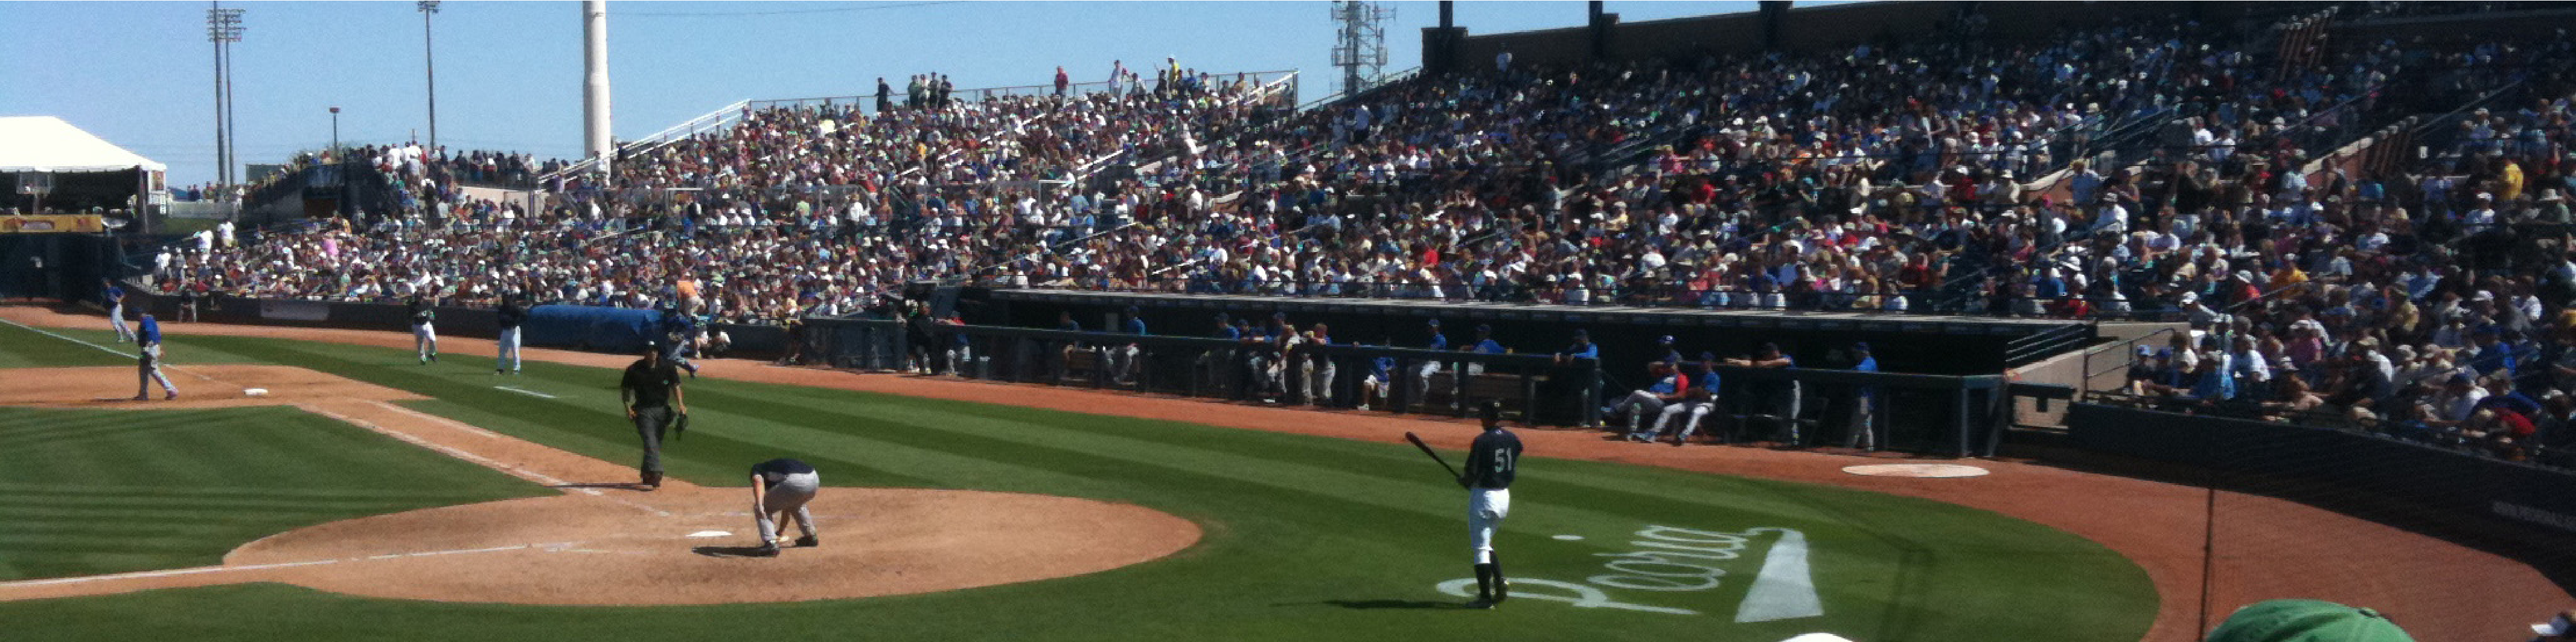
\includegraphics[width=\textwidth]{sampleteaser}
  \caption{This is a teaser}
  \label{fig:teaser}
\end{teaserfigure}


\maketitle

$body$

\bibliographystyle{ACM-Reference-Format}
\bibliography{my-bibliography}

\end{document}
